\documentclass{article}

\usepackage{graphicx}
\usepackage{listings}
\usepackage{color}
\usepackage{hyperref}
\usepackage{float}

\definecolor{dkgreen}{rgb}{0,0.6,0}
\definecolor{gray}{rgb}{0.5,0.5,0.5}
\definecolor{mauve}{rgb}{0.58,0,0.82}

\lstset{frame=tb,
  language=C++,
  aboveskip=3mm,
  belowskip=3mm,
  showstringspaces=false,
  columns=flexible,
  basicstyle={\small\ttfamily},
  numbers=none,
  numberstyle=\tiny\color{gray},
  keywordstyle=\color{blue},
  commentstyle=\color{dkgreen},
  stringstyle=\color{mauve},
  breaklines=true,
  breakatwhitespace=true,
  tabsize=3
}

\begin{document}

    \title{%
      Metaballs in GLFW \\
      \large DD2323 Project Report \\}

    \author{Alexander Hjelm (alhjelm@kth.se), Tsz Kin Chan (XXXXXXXXXXXXXXXXx@kth.se)}

    \date{\today}

    \maketitle

    \section{Summary}
    Hippety hoppety, Women are property! >:)
    
    \section{Introduction}
    
    Metaballs are soft, organic-looking 3D objects that appear to blob together when they are very close, and can be used to simulate dynamic fluids if using many particles on a large simulation domain. 
    The metaballs rendering technique was invented by Jim Blinn in the early 1980s, and has been a very common demo effect since the 1990s.

    The metaballs model is defined as a 3D isosurface, and can be rendered using the same methods that are common to isosurfaces.
    The most common methods for rendering metaballs are ray-tracing for still image and animations, and the marching cubes algorithm for real time.

    [https://steve.hollasch.net/cgindex/misc/metaballs.html]

    \begin{figure}[H]
        \begin{center}
        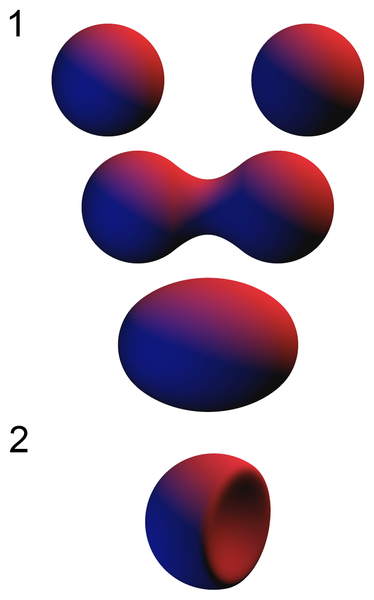
\includegraphics[width=0.4\linewidth]{img/metaballs-concept.png}
        \caption{A conceptual visualisation of how metaballs work. Part 1 shows two metaballs gradually merging, and part 2 shows the influence of a negative metaball on a positive metaball.}
        \label{fig:metaballs-concept}
        \end{center}
    \end{figure}
    [https://en.wikipedia.org/wiki/File:Metaballs.png]

    Using low-level graphics programming, we have programmed and rendered a real time, dynamic fluid using the metaballs with the marching cubes technique. The fluid particles use a basic physics model to collide with each other and the environment.
    This report will present the theory behind the metaballs rendering technique and show how it can be implemented as a real time simulation.

    \section{Theory}

        \subsection{Metaball isosurface model}
            A metaball is an isosurface in 3D space. 
            Define a function $f(x,y,z)$, which takes as input a set of coordinates in 3D space, and returns a floating poing value that represents the influence of the function on that point.
            When we have such a function, we can sample it at even or random intervals to determine which points belong inside the surface and which belong outside it.
            This is simply a matter of comparing wether the influence at a point is greater than a fixed threshold or not.
            We can then use a number of different rendering techniques to create a presentation of this 3D surface, as we shall see in the next section.

            For now, let us look at the metaball surface model in particular. The most common isosurface fucntion for the metaball model is inverse quadratic:

            $[f(x,y,z) = 1.0 / (x^2 + y^2 + z^2)]$

            This function describes a field where each ball has an influence point with quadratic falloff.
            For any point $\vec{p}$ in 3D, and for any ball's position $\vec{b}$, the influence of that ball on the point $\vec{p}$ will be proporitonal to $|\vec{p} - \vec{b}|^2$.
            This function is also used to model the strength of electrical fields in electromagnetics, which is why we choose to label it as the metaball potetial field function.
            [http://www.geisswerks.com/ryan/BLOBS/blobs.html]

            If one were to draw the resulting field of a single metaball around the origin, it might look like figure 2, where the brightness of the color indicates the influence of the field at that point.
            
            \begin{figure}[H]
                \begin{center}
                
\includegraphics[width=0.6\linewidth]{img/2d-potential.png}
                \caption{A concept of the inverse square function in 2D}
                \label{fig:2d-potential}
                \end{center}
            \end{figure}

            A similar model for two metaballs, with their potential fields partially overlapping in different stages, is shown in figure 3.
            
            \begin{figure}[H]
                \begin{center}
                
\includegraphics[width=\linewidth]{img/2d-potential-multi.png}
                \caption{A concept of 2 metaballs in 2D. Every frame shows the two balls moving closer to each other.}
                \label{fig:2d-potential-multi}
                \end{center}
            \end{figure}

            As you can see, the area between the two balls becomes gradually lit up.
            The intersection between the two potetial fields becomes brighter as the two balls move closer, and at some point the center point between the balls will have a strength that is above our threshold. This effect will propagate outwards as the balls move closer, and we will use this later to make the balls appear as if they blob together in 3D.

        \subsection{Marching cubes}
            Voxel shader with an array of predefined cube shapes. The shader selects the relevant cube shape depending on how the neighbourhood looks with respect to the potential.

    \section{Implementation}

        We have used GLFW and GLSL. GLFW is a utility library for working with OpenGL, and we will use it as an interface between the high-level program logic and the low-level rendering. Mainly we will use GLFW to manage the OpenGL context and make GPU drawcalls. GLSL is the OpenGL shading language that gives developers control over the rendering pipeline. We will use GLSL to write our shader programs.

        \begin{lstlisting}
        private void Test(){
            int a = 1;
        }
        \end{lstlisting}

        \subsection{Misc}
            For the purpose of creating a nice demo, we created a fragment shader with basic Phong illumination, in order to give the animation more depth.
            We also added a physics model to the balls which consists of outer forces due to gravity and a repelling force between each pair of balls when they are close to each other, to prevent them from accumulating in one place.
            We also modelled the bounciness of the floor and walls of our simulation domain, in order to keep the balls confined and in motion for as long as possible.

            We will not go into the details of how we implemented physics and the illumination model, as they are out of the focus of this report.

    \section{Result}
        \begin{figure}[H]
            \begin{center}
            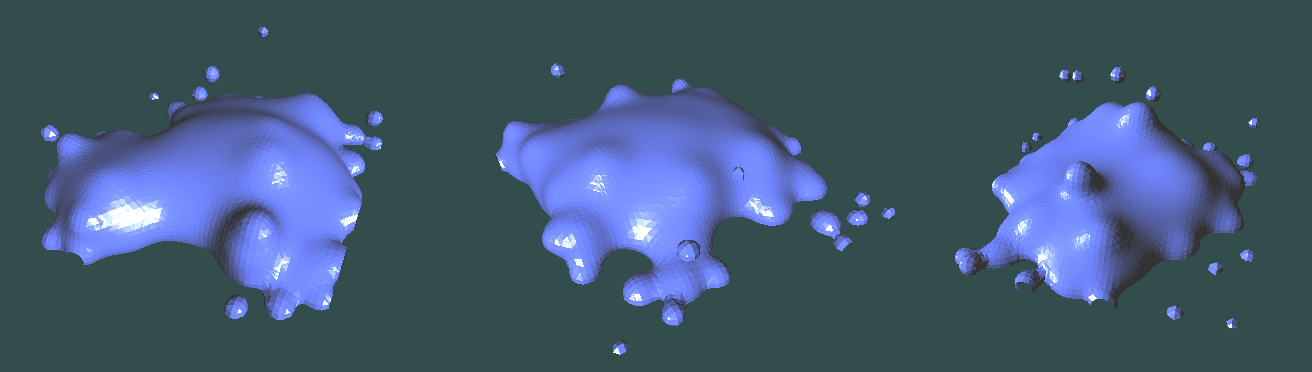
\includegraphics[width=\linewidth]{img/result-animation.png}
            \caption{A concept of 2 metaballs in 2D. Every frame shows the two balls moving closer to each other.}
            \label{fig:result-animation}
        \end{center}
        \end{figure}

        An animated video can be found here:
        \url{https://youtu.be/jmScNqchXs0}

    \section{Conclusions}
    
        \subsection{Rendering model}
        The voxel grid size is the performance bottleneck.

        Comparison.
        Number of metaballs vs the maximum voxel grid size before the framerate drops below 30:

        \begin{tabular}{ l | c | r }
          50 & 120 \\
          20 & 160 \\
          5 & 200 \\
        \end{tabular}

        Disabling the metaball filter completely, and just running the voxel shader yields a maximum voxel grid size of 310 units before the framrate drops below 30.

        The test was run on a NVIDIA Geforce GTX 1050 Ti.

        Conclusion: The geometry shader itself can run with a voxel grid size in the order of 100-200 units at 60 fps, and up to 300 units at 30 fps.
        For our purpose, this can be used to create a nice looking dynamic fluid on a small simulation domain, or a very chunky fluid on a medium-large sized simulation domain.
        To render an impressive fluid in a medium sized voxel grid, it would be nice if we could optimize the particle model so that we could run in the order of 100 particles at a voxel grid size of 200.
        The following section will discuss some ideas for how this could be achieved in theory.

        \subsection{Particle model}
    	It seems that the industry standard for fluid simulation in high quality games and video is the Smoothed Particle Hydrodynamics model with Ellipsoid Splatting rendering.
        Right now we are brute forcing the potential field over all particles
        (Possible conslusion: in line with SPH: spatial subdivision of metaball positions will allow for more balls, but not yield the neccessary performance increase that is needed to simulate particles in a high-resolution domain)

        Yet another performance problem comes from the fact that the division step in our metaball potential function is computationally expensive.
        Ryan Geiss (whose tutorial on the metaball isosurface model we used) came with a suggestion for an approximate polynomial function which should in theory be faster on the GPU. His suggested function was:

        $[g(r) = r^4 - r^2 + 0.25]$

        This potential field function also has the neat property that it evaluates to 0 at $r=\frac{1}{\sqrt{2}}$, which means that you could do spatial optimization by only evaulating the points that fall within the radius of $r=\frac{1}{\sqrt{2}}$ of a singe metaball's center.

        [http://www.geisswerks.com/ryan/BLOBS/blobs.html]

        Our prediction is that this would yield a similar performance increase to implementing a naive spacial subdivision, but we are still not solving the problem that the geometry shader itself is expensive.

\end{document}
